%%%%%%%%%%%%%%%%%%%%%%%%%%%%%%%%%%%%%%%%%
% Beamer Presentation
% LaTeX Template
% Version 1.0 (10/11/12)
%
% This template has been downloaded from:
% http://www.LaTeXTemplates.com
%
% License:
% CC BY-NC-SA 3.0 (http://creativecommons.org/licenses/by-nc-sa/3.0/)
%
%%%%%%%%%%%%%%%%%%%%%%%%%%%%%%%%%%%%%%%%%

%----------------------------------------------------------------------------------------
%	PACKAGES AND THEMES
%----------------------------------------------------------------------------------------

\documentclass{beamer}
\usepackage{listings}
\mode<presentation> {
\usetheme{Madrid}
}

\usepackage{graphicx} % Allows including images
\usepackage{booktabs} % Allows the use of \toprule, \midrule and \bottomrule in tables

%----------------------------------------------------------------------------------------
%	TITLE PAGE
%----------------------------------------------------------------------------------------

\title[Short title]{A CS251 Project Report
by Group 11.} % The short title appears at the bottom of every slide, the full title is only on the title page
%author{N Divakar Reddy} % Your name
\author[N Divakar Reddy \& Y Pushyarag  \& Vishal Babu Bhavani]
{%
  \texorpdfstring{
    \begin{columns}%[onlytextwidth] 
      \column{.30\linewidth}
      \centering
      N Divakar Reddy\\
      140050044\\
      divakar@cse.iitb.ac.in
      \column{.30\linewidth}
      \centering
      Y Pushyarag\\ 
      140050047\\
      pushyarag@cse.iitb.ac.in
      \column{.30\linewidth}
      \centering
      Vishal Babu Bhavani\\
      140050049\\
      johnpete@cse.iitb.ac.in
    \end{columns}
  }
  {N Divakar Reddy \& Y Pushyarag  \& Vishal Babu Bhavani}
}

%----------------------------------------------------------------------------------------
\date{\today} % Date, can be changed to a custom date

%----------------------------------------------------------------------------------------

\begin{document}

\begin{frame}
\titlepage % Print the title page as the first slide
\end{frame}

\begin{frame}
\frametitle{Overview} % Table of contents slide, comment this block out to remove it
\tableofcontents % Throughout your presentation, if you choose to use \section{} and \subsection{} commands, these will automatically be printed on this slide as an overview of your presentation
\end{frame}

%----------------------------------------------------------------------------------------
%	PRESENTATION SLIDES
%----------------------------------------------------------------------------------------
\section{Introduction}
\begin{frame}
\frametitle{Introduction}
\begin{itemize}
\item This report is made to describe the concepts behind our CS251
project Box2d simulation.
\item  In this project we have created a simulation of a Rube Goldberg machine we designed, in C++ using the Box2D library.
\item  A Rube Goldberg machine is a contraption that performs a simple task in a complicated fashion.
\end{itemize}
\end{frame}

%------------------------------------------------


\section{Motivation}
\begin{frame}
\frametitle{Motivation}
\begin{itemize}
\item Our motivation of doing this project is our curiosity to learn box2d,and get hands on it.
\item Our main motive of doing this project is to get to know and work with a lot of new stuff like
box2d,makefiles,etc
\item we will be doing the project before the midsem.
\end{itemize}
\end{frame}





%------------------------------------------------

%------------------------------------------------

\section{Description}



\begin{frame}
\frametitle{Description}
\begin{itemize}
\item The project has many objects like dominoes, blocks, spheres, rotating planks and pulleys.
\item Once the time is 6:00 A.M. the simulation starts and continues involving all the objects used in the project and ends with water falling on a sleeping guy.
\begin{figure}
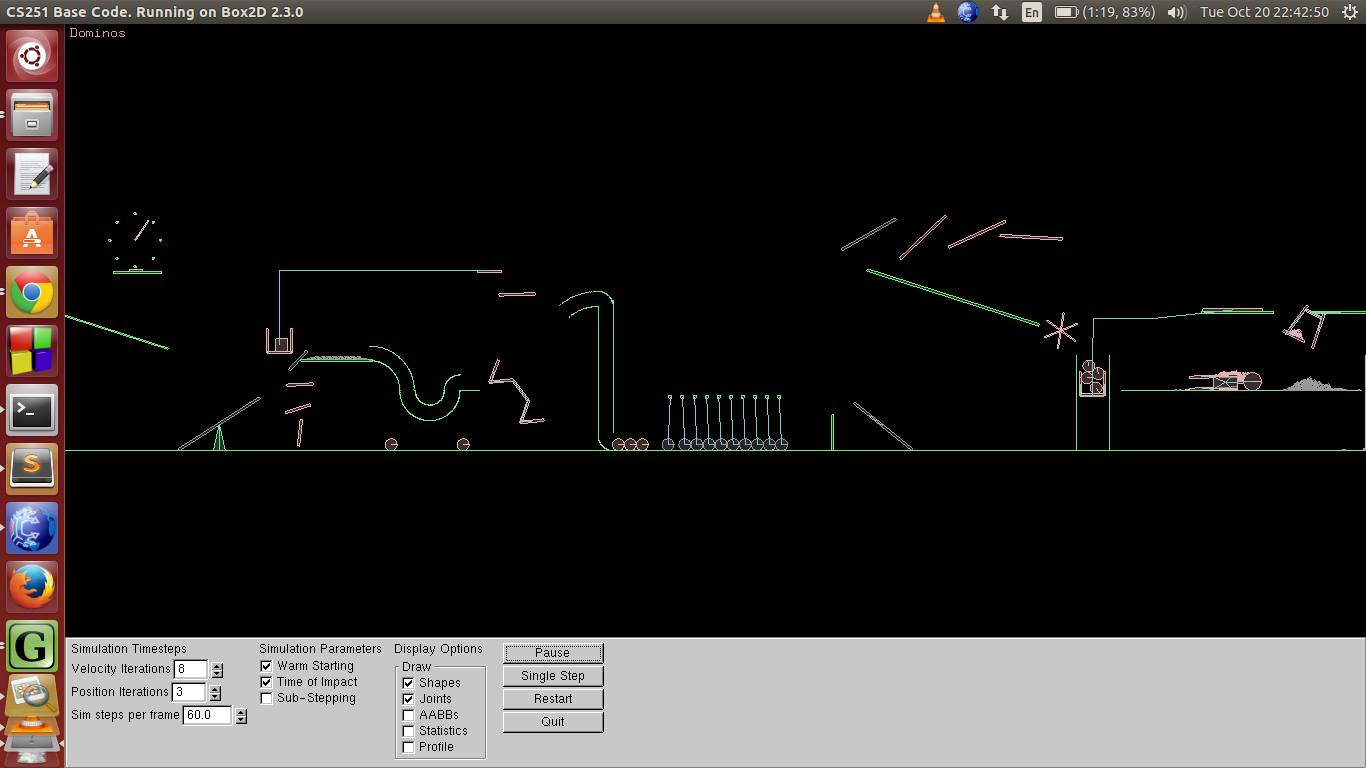
\includegraphics[width=0.8\linewidth]{screen.png}
\end{figure}
\end{itemize}
\end{frame}




















\end{document}